\documentclass[tikz,border=2pt]{standalone}
\usepackage{amsmath,amssymb}
\usepackage{tikz}
\usetikzlibrary{arrows.meta,calc,positioning}

\begin{document}
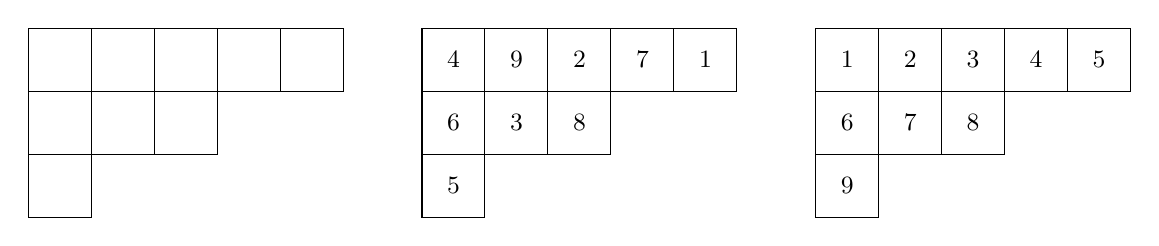
\begin{tikzpicture}[>=Stealth]
  % Global box size and text style
  \def\bs{0.8} % box size in cm
  \tikzset{
    cell/.style = {draw, minimum width=\bs cm, minimum height=\bs cm, inner sep=0pt, outer sep=0pt, anchor=south west},
    lab/.style  = {font=\footnotesize},
    num/.style  = {font=\small}
  }

  % We'll work in integer grid units scaled by \bs for convenient placement
  \begin{scope}[x=\bs cm,y=\bs cm]

    % ========= Panel 1: Empty Young diagram λ=(5,3,1) =========
    % top row (length 5) at y=2
    \foreach \x in {0,1,2,3,4} { \node[cell] at (\x,2) {}; }
    % middle row (length 3) at y=1
    \foreach \x in {0,1,2}     { \node[cell] at (\x,1) {}; }
    % bottom row (length 1) at y=0
    \node[cell] at (0,0) {};
    % title
    % \node[lab, align=center] at (2, -0.8) {Young diagram\\$\lambda=(5,3,1)$};

    % ========= Panel 2: Young tableau with random entries =========
    % Shift this panel to the right by +4 grid units
    \begin{scope}[xshift=4cm/\bs] % note: converts cm to grid units
      % draw boxes (same shape)
      \foreach \x in {0,1,2,3,4} { \node[cell] at (\x,2) {}; }
      \foreach \x in {0,1,2}     { \node[cell] at (\x,1) {}; }
      \node[cell] at (0,0) {};
      % random numbers placed row-wise (choose any permutation of 1..9)
      % top row y=2: 5 boxes
      \node[num] at (0.5,2.5) {4};
      \node[num] at (1.5,2.5) {9};
      \node[num] at (2.5,2.5) {2};
      \node[num] at (3.5,2.5) {7};
      \node[num] at (4.5,2.5) {1};
      % middle row y=1: 3 boxes
      \node[num] at (0.5,1.5) {6};
      \node[num] at (1.5,1.5) {3};
      \node[num] at (2.5,1.5) {8};
      % bottom row y=0: 1 box
      \node[num] at (0.5,0.5) {5};
      % title
      % \node[lab, align=center] at (2, -0.8) {Young tableau (random)};
    \end{scope}

    % ========= Panel 3: Standard Young tableau (row-wise 1..n) =========
    \begin{scope}[xshift=8cm/\bs]
      % draw boxes (same shape)
      \foreach \x in {0,1,2,3,4} { \node[cell] at (\x,2) {}; }
      \foreach \x in {0,1,2}     { \node[cell] at (\x,1) {}; }
      \node[cell] at (0,0) {};
      % row-wise fill with 1..9 (this is standard for λ=(5,3,1))
      % top row (y=2)
      \node[num] at (0.5,2.5) {1};
      \node[num] at (1.5,2.5) {2};
      \node[num] at (2.5,2.5) {3};
      \node[num] at (3.5,2.5) {4};
      \node[num] at (4.5,2.5) {5};
      % middle row (y=1)
      \node[num] at (0.5,1.5) {6};
      \node[num] at (1.5,1.5) {7};
      \node[num] at (2.5,1.5) {8};
      % bottom row (y=0)
      \node[num] at (0.5,0.5) {9};
      % title
      % \node[lab, align=center] at (2, -0.8) {Standard Young tableau};
    \end{scope}

  \end{scope}
\end{tikzpicture}
\end{document}
